\section{Graphs of Evaluation Functions} \label{Graphs}

The method described in this article tries to learn evaluation functions of association measures by graphical means. The first attempt to explore the quantifiers was to plot them with suitable graphical tools. One can only draw graphs of functions that contain two or three independent variables. In case of three independent variables, we chose one of the variables (the least significant) as parameter and draw graphs of two remaining variables while changing the parameter. 

Although work described in this section was done mainly to get familiarized with functions and did not contain any special theory, we obtained one interesting result. It is the comparison of the {\it founded equivalence \/}
and {\it pairing \/} quantifiers. The {\it pairing \/} quantifier is defined only by $a$ and
$d$, {\it founded equivalence \/} uses additionally $n$, size of the contingency table. We used
$n$ as parameter for the graph. The two graphs can be seen in figure \ref{fig:FEPairing}.

\begin{figure}[ht]
\centering
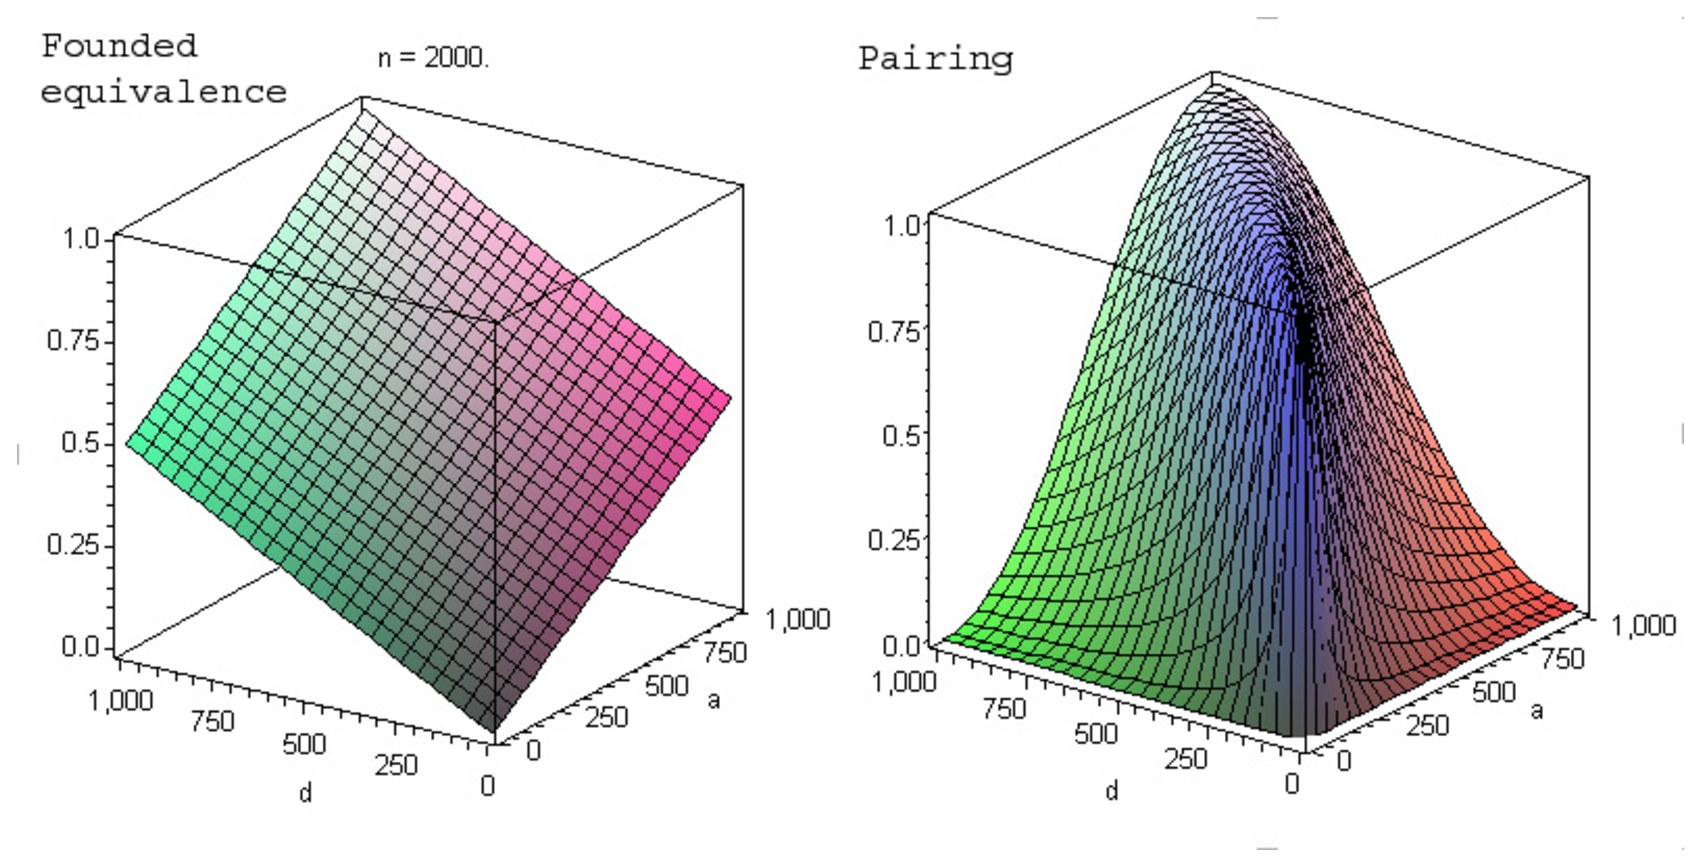
\includegraphics[width=115mm]{FE-Pairing.eps}
%\mbox{\resizebox{125mm}{!}{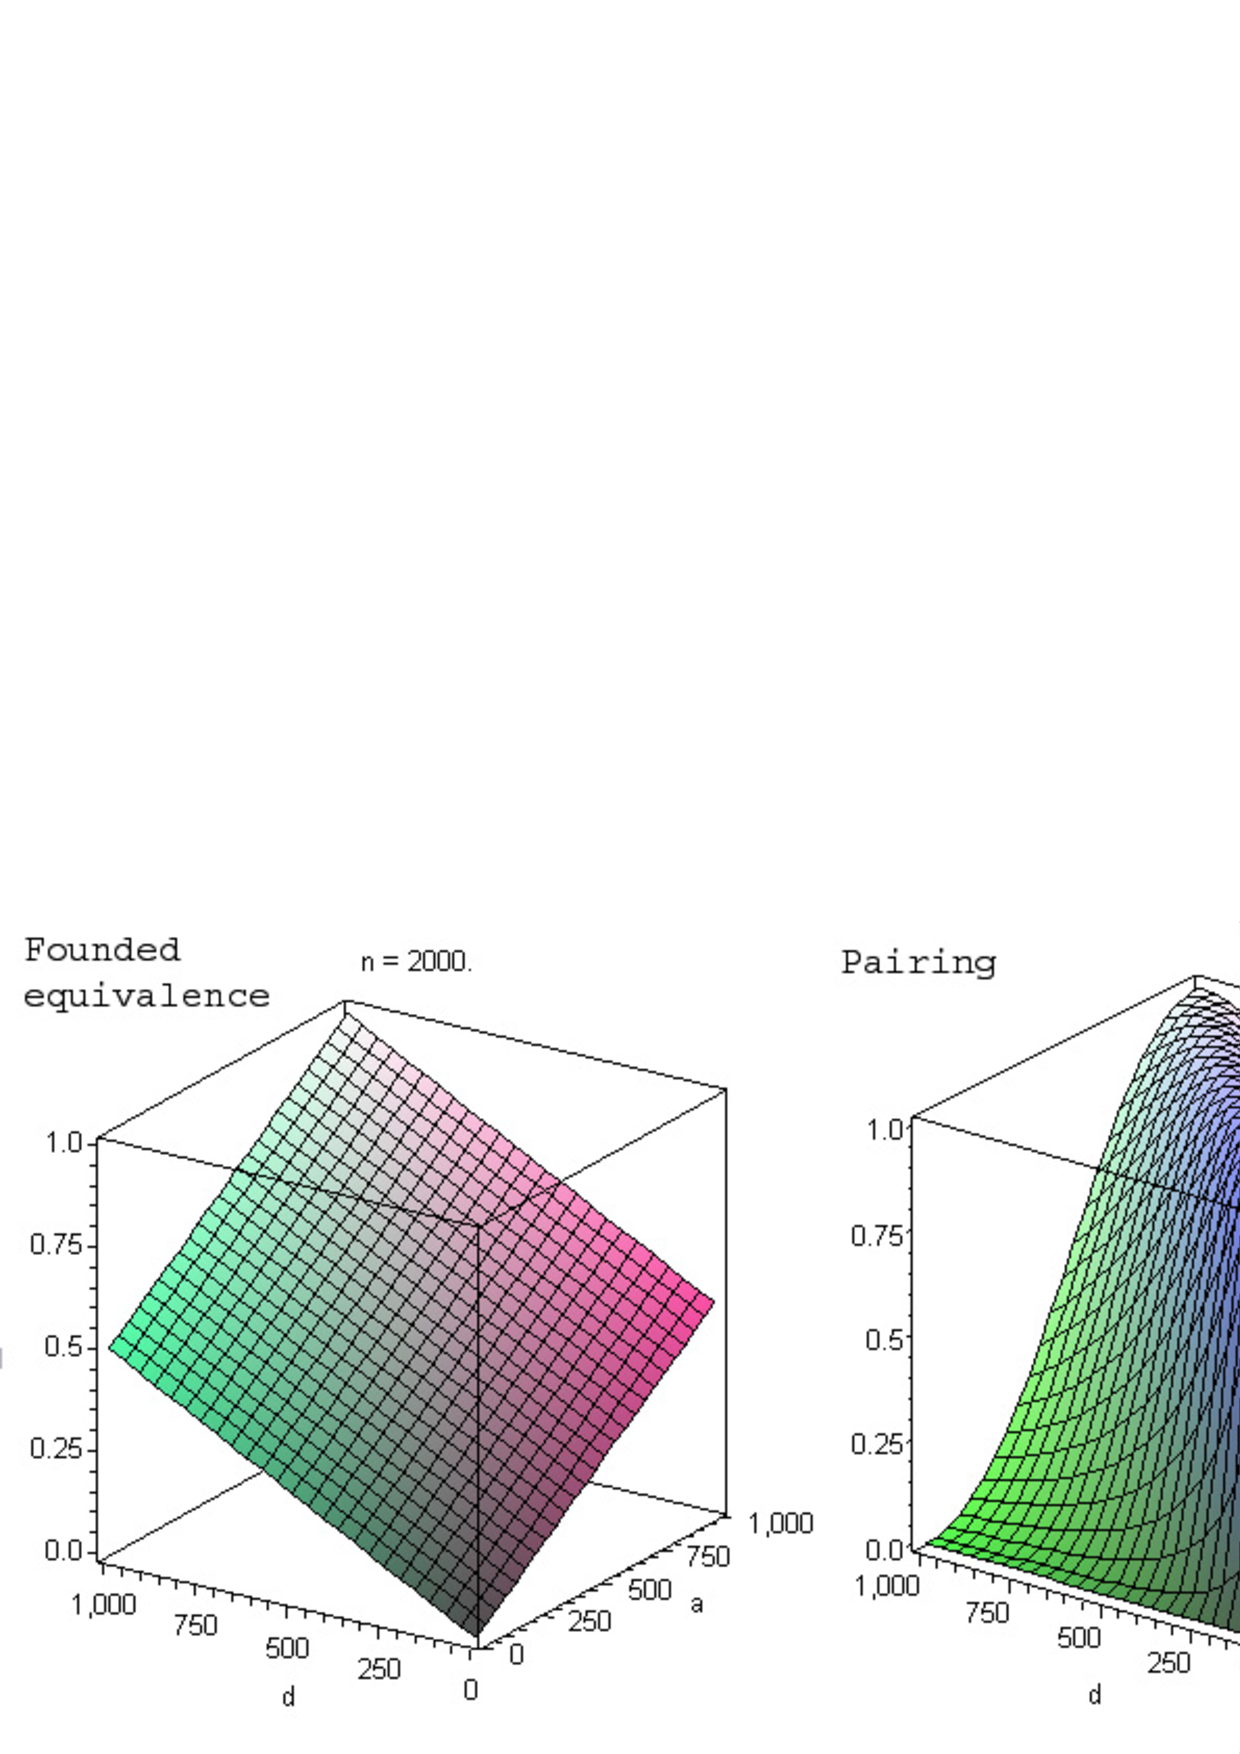
\includegraphics{FE-Pairing.png}}}
\caption{Founded equivalence and Pairing quantifiers graphs}
\label{fig:FEPairing}
\end{figure}

Semantics of the quantifier is stated by its evaluation function. However, the formula for 
{\it pairing \/} quantifier is too complex to be comprehended. Therefore it is suitable to examine graph of this quantifier and compare it to the graph of the {\it founded equivalence \/}, because these two quantifiers use same variables ($a$ and $d$). 

The {\it founded equivalence \/} graph is a plane that increases with $a$ and $d$ and its slope is determined by $n$. Contrary, the {\it pairing \/} quantifier's graph is a "ridge" above the $a d$ diagonal. Then, the characterizing property of the {\it founded equivalence \/} is \emph{the bigger a+d, the better}\footnote{This was apparent also from the evaluation function.} and for {\it pairing \/} quantifier \emph{the closer a is to d, the better}.

Both quantifiers have disadvantages: {\it founded equivalence \/} is unable to distinguish between $a$ and $d$. This fact reveals common misunderstanding of equivalence quantifiers:
although it may seem that equivalence is a stronger implication, for {\it implicational \/}
and {\it equivalence \/} classes of quantifiers, it is not the case.
The {\it pairing \/} quantifier on the other hand is unable to consider $b$ and $c$, thus resulting rule may be weakly supported. 

The analysis shows us how to use both quantifiers in a more profound way. When using {\it founded equivalence \/}, we should also look at the ratio of $a/d$ to see how good the rule is in terms of positive and negative examples. We should use {\it pairing \/} quantifier to find balanced all-positive, all-negative examples ratio; it is preferable to aid
with the {\it founded equivalence \/} evaluation function. This new perception of the two quantifiers was made possible mainly by examining their graphs.

\medskip

One of the initial motivations was to somehow express the \emph{founded implication}, \emph{lower critical implication }and \emph{upper critical implication} from the same point of view. Graph of functions do not help, because the only way to graph critical implications is to set $p$ as parameter, which makes them incomparable to the \emph{founded implication}, where the $p$ is value of two-dimensional function. This problem is solved in section \ref{Graphs_Tables} by displaying graphs of critical frequencies of quantifiers. 